% !TeX encoding = UTF-8
% !TeX program = pdflatex
% !BIB program = biber

\documentclass[
        english,biblatex
    ]{lni}

\addbibresource{my-paper.bib}


% Standard packages
\usepackage{graphicx}
\usepackage{longtable}
\usepackage{booktabs}
\usepackage{array}
\usepackage{multirow}
\usepackage{wrapfig}
\usepackage{float}
\usepackage{colortbl}
\usepackage{pdflscape}
\usepackage{tabularx}
\usepackage{threeparttable}
\usepackage{threeparttablex}
\usepackage[normalem]{ulem}
\usepackage{makecell}

\usepackage{framed} % Needed for code blocks

\usepackage{color}
\usepackage{fancyvrb}
\newcommand{\VerbBar}{|}
\newcommand{\VERB}{\Verb[commandchars=\\\{\}]}
\DefineVerbatimEnvironment{Highlighting}{Verbatim}{commandchars=\\\{\}}
% Add ',fontsize=\small' for more characters per line
\usepackage{framed}
\definecolor{shadecolor}{RGB}{241,243,245}
\newenvironment{Shaded}{\begin{snugshade}}{\end{snugshade}}
\newcommand{\AlertTok}[1]{\textcolor[rgb]{0.68,0.00,0.00}{#1}}
\newcommand{\AnnotationTok}[1]{\textcolor[rgb]{0.37,0.37,0.37}{#1}}
\newcommand{\AttributeTok}[1]{\textcolor[rgb]{0.40,0.45,0.13}{#1}}
\newcommand{\BaseNTok}[1]{\textcolor[rgb]{0.68,0.00,0.00}{#1}}
\newcommand{\BuiltInTok}[1]{\textcolor[rgb]{0.00,0.23,0.31}{#1}}
\newcommand{\CharTok}[1]{\textcolor[rgb]{0.13,0.47,0.30}{#1}}
\newcommand{\CommentTok}[1]{\textcolor[rgb]{0.37,0.37,0.37}{#1}}
\newcommand{\CommentVarTok}[1]{\textcolor[rgb]{0.37,0.37,0.37}{\textit{#1}}}
\newcommand{\ConstantTok}[1]{\textcolor[rgb]{0.56,0.35,0.01}{#1}}
\newcommand{\ControlFlowTok}[1]{\textcolor[rgb]{0.00,0.23,0.31}{\textbf{#1}}}
\newcommand{\DataTypeTok}[1]{\textcolor[rgb]{0.68,0.00,0.00}{#1}}
\newcommand{\DecValTok}[1]{\textcolor[rgb]{0.68,0.00,0.00}{#1}}
\newcommand{\DocumentationTok}[1]{\textcolor[rgb]{0.37,0.37,0.37}{\textit{#1}}}
\newcommand{\ErrorTok}[1]{\textcolor[rgb]{0.68,0.00,0.00}{#1}}
\newcommand{\ExtensionTok}[1]{\textcolor[rgb]{0.00,0.23,0.31}{#1}}
\newcommand{\FloatTok}[1]{\textcolor[rgb]{0.68,0.00,0.00}{#1}}
\newcommand{\FunctionTok}[1]{\textcolor[rgb]{0.28,0.35,0.67}{#1}}
\newcommand{\ImportTok}[1]{\textcolor[rgb]{0.00,0.46,0.62}{#1}}
\newcommand{\InformationTok}[1]{\textcolor[rgb]{0.37,0.37,0.37}{#1}}
\newcommand{\KeywordTok}[1]{\textcolor[rgb]{0.00,0.23,0.31}{\textbf{#1}}}
\newcommand{\NormalTok}[1]{\textcolor[rgb]{0.00,0.23,0.31}{#1}}
\newcommand{\OperatorTok}[1]{\textcolor[rgb]{0.37,0.37,0.37}{#1}}
\newcommand{\OtherTok}[1]{\textcolor[rgb]{0.00,0.23,0.31}{#1}}
\newcommand{\PreprocessorTok}[1]{\textcolor[rgb]{0.68,0.00,0.00}{#1}}
\newcommand{\RegionMarkerTok}[1]{\textcolor[rgb]{0.00,0.23,0.31}{#1}}
\newcommand{\SpecialCharTok}[1]{\textcolor[rgb]{0.37,0.37,0.37}{#1}}
\newcommand{\SpecialStringTok}[1]{\textcolor[rgb]{0.13,0.47,0.30}{#1}}
\newcommand{\StringTok}[1]{\textcolor[rgb]{0.13,0.47,0.30}{#1}}
\newcommand{\VariableTok}[1]{\textcolor[rgb]{0.07,0.07,0.07}{#1}}
\newcommand{\VerbatimStringTok}[1]{\textcolor[rgb]{0.13,0.47,0.30}{#1}}
\newcommand{\WarningTok}[1]{\textcolor[rgb]{0.37,0.37,0.37}{\textit{#1}}}

% solve \tightlist error
\providecommand{\tightlist}{%
    \setlength{\itemsep}{0pt}\setlength{\parskip}{0pt}}

% solve \pandocbounded error
\providecommand{\pandocbounded}[1]{#1}



\begin{document}

% Title
        \title[]{The difference between RSE and Data Science}
    
    
    


\author[1]{Julian Dehne}{julian.dehne@gi.de}{0000-0001-9265-9619}
\author[2]{Jan Philipp Thiele}{jan-philipp.thiele@tu-braunschweig.de}{0000-0002-8901-6660}
\author[3]{Jeremy Cohen}{jeremy.cohen@imperial.ac.uk}{0000-0003-4312-2537}
\author[4]{Katrin Schöning-Stierand}{\href{mailto:katrin.schoening-stierand@uni-hamburg.de}{katrin.schoening-stierand@uni-hamburg.de}}{0000-0003-3248-8023}
\author[5]{Florian Goth}{\href{mailto:Florian.Goth@uni-wuerzburg.de}{Florian.Goth@uni-uerzburg.de}}{0000-0003-2707-4790}
\author[6]{Jan Linxweiler}{\href{mailto:j.linxweiler@tu-braunschweig.de}{j.linxweiler@tu-braunschweig.de}}{0000-0002-2755-5087}
\author[7]{Anna-Lena Lamprecht}{\href{mailto:anna-lena.lamprecht@uni-potsdam.de}{anna-lena.lamprecht@uni-potsdam.de}}{0000-0003-1953-5606}

\affil[1]{Gesellschaft für Informatik\\Bildung und Gesellschaft\\
Weydingerstraße 14-16\\10178 Berlin\\Deutschland}
\affil[2]{TU Braunschweig\\Universitätsbibliothek\\
Universitätspl. 1, 38106 Braunschweig\\Deutschland}
\affil[3]{University 3\\Department\\Address\\Country}
\affil[4]{Universität Hamburg\\Hub of Computing and Data Science\\Albert-Einstein-Ring 8\\22761 Hamburg\\Deutschland}
\affil[5]{Universität Würzburg\\Institut für theoretische Physik 1\\Am Hubland\\97070 Würzburg\\Deutschland}
\affil[6]{TU Braunschweig\\Universitätsbibliothek\\
Universitätspl. 1, 38106 Braunschweig\\Deutschland}
\affil[7]{Universität Potsdam\\Chair of Software Engineering\\An der Bahn 2\\14476 Potsdam\\Deutschland}


    \maketitle

% Abstract
        \begin{abstract}
        Die LaTeX-Klasse \texttt{lni} setzt die Layout-Vorgaben für
        Beiträge in LNI Konferenzbänden um. Dieses Dokument beschreibt
        ihre Verwendung und ist ein Beispiel für die entsprechende
        Darstellung.
    \end{abstract}
    
% Keywords
        \begin{keywords}
        LNI Guidelines \and LaTeX Vorlage
    \end{keywords}
    
% Body
    \section{Verwendung}\label{verwendung}

    Die GI gibt unter http://www.gi-ev.de/LNI Vorgaben für die
    Formatierung von Dokumenten in der LNI Reihe.

    \section{Demonstrationen}\label{demos}

    \section{Demonstration der Einhaltung der
    Richtlinien}\label{lniconformance}

    \subsection{Literaturverzeichnis}\label{literaturverzeichnis}

    Beispielhafte Zitierungen: \textcite{Ez10}, \textcite{AB00}.

    \section{Abbildungen}\label{abbildungen}

    \begin{figure}

    \centering{

    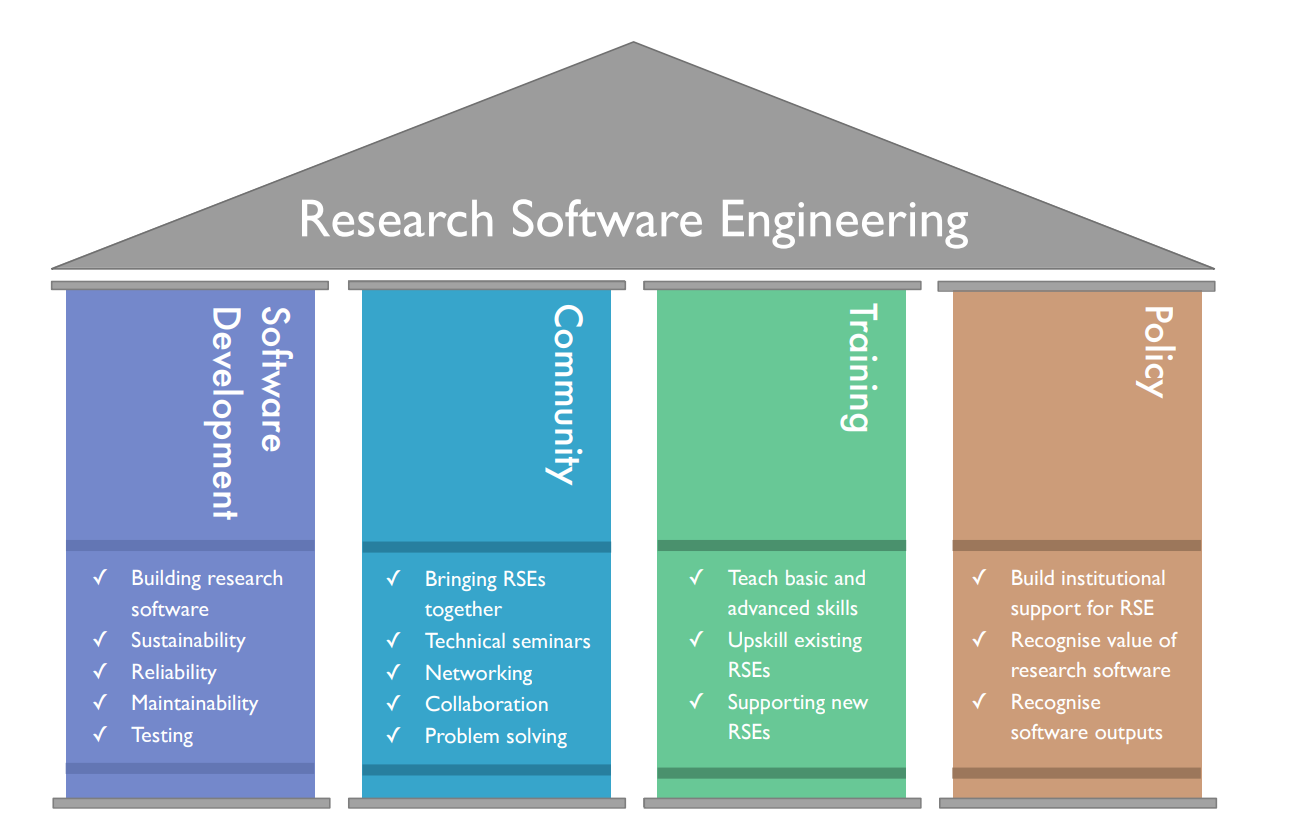
\includegraphics[width=0.8\linewidth,height=\textheight,keepaspectratio]{four_pillars_rse.png}

    }

    \caption{\label{fig-demo}Demographik}

    \end{figure}%

    \section{Tabellen}\label{tabellen}

    \begin{longtable}[]{@{}lll@{}}
    \caption{Die Überschriftsarten \{\#tab-demo\}}\tabularnewline
    \toprule\noalign{}
    Überschriftsebenen & Beispiel & Schriftgröße und -art \\
    \midrule\noalign{}
    \endfirsthead
    \toprule\noalign{}
    Überschriftsebenen & Beispiel & Schriftgröße und -art \\
    \midrule\noalign{}
    \endhead
    \bottomrule\noalign{}
    \endlastfoot
    Titel (linksbündig) & Der Titel \ldots{} & 14 pt, Fett \\
    Überschrift 1 & 1 Einleitung & 12 pt, Fett \\
    Überschrift 2 & 2.1 Titel & 10 pt, Fett \\
    \end{longtable}

    \section{Programmcode}\label{programmcode}

\begin{Shaded}
\begin{Highlighting}[]
\KeywordTok{public} \KeywordTok{class}\NormalTok{ Hello }\OperatorTok{\{}
    \KeywordTok{public} \DataTypeTok{static} \DataTypeTok{void} \FunctionTok{main} \OperatorTok{(}\BuiltInTok{String}\OperatorTok{[]}\NormalTok{ args}\OperatorTok{)} \OperatorTok{\{}
        \BuiltInTok{System}\OperatorTok{.}\FunctionTok{out}\OperatorTok{.}\FunctionTok{println}\OperatorTok{(}\StringTok{"Hello World!"}\OperatorTok{);}
    \OperatorTok{\}}
\OperatorTok{\}}
\end{Highlighting}
\end{Shaded}

    \section{What has been discussed}\label{what-has-been-discussed}

    TODO insert: Levels of Differences between RSE and DS:

    \begin{itemize}
    \tightlist
    \item
      institutional
    \item
      disciplinary connections
    \item
      target groups
    \item
      political history
    \end{itemize}

    \section{RSE and DS embeddings in the Research
    Cycle}\label{rse-and-ds-embeddings-in-the-research-cycle}

    Both RSE and DS can be conceptualized as a cross-cutting concern in
    many disciplines. However, the definition and relevance of these
    issues can be generalized based on the function they fulfill in the
    research cycle Figure~\ref{fig-research_cycle}.

    \newpage

    \begin{figure}

    \centering{

    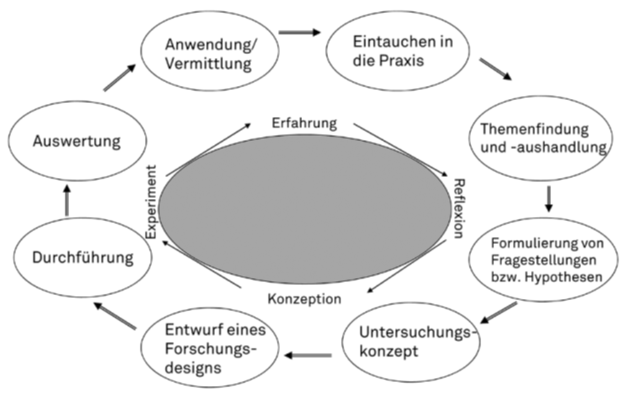
\includegraphics[width=0.7\linewidth,height=\textheight,keepaspectratio]{img/research_cycle_wildt.png}

    }

    \caption{\label{fig-research_cycle}The research cycle
    \autocite{wildt2009forschendes} integrates the typical research
    process with the learning process.}

    \end{figure}%

    There are different research processes depending on the discipline
    and the research question. However, \autocite{Dehne2021} showed that
    most of the research processes contain the following phases:

    \begin{enumerate}
    \def\labelenumi{\arabic{enumi}.}
    \tightlist
    \item
      conceptualization (developing research questions, concepts)
    \item
      design (developing the tools, instruments and concrete process
      models)
    \item
      implementation (executing the experiment, study)
    \item
      analysis \& interpretation
    \item
      dissemination (publishing, distributing, peer-review)
    \item
      reflexion and improvements
    \end{enumerate}

    For example, in the case of the field of learning technologies, the
    design phase often consists of extensive software development of
    different tools for learning. In this situation developing complex
    tools for learning can be considered as research software
    engineering. The analysis of what learners can gain from using these
    technologies can be conceived as an educational research in its own
    right. This example highlights the differences of scale in both the
    weight of the different process phases (here: phase 2) and the
    relevance of research engineering. It also shows a situation where
    research software engineering clearly differs from data science. A
    typical data science background would not enable researchers to
    build full-stack software that solves inefficiencies or
    hard-to-teach problems in education.

    In the second example a GPT-like attention model is trained to
    classify data gained from the James-Webb telescope. Due to vast
    amounts of data and the continuous stream of new data research
    software engineering is needed to implement a pipeline for data
    cleaning, data warehousing and in-time analysis. In this case, the
    analysis \& interpretation phase (4) has much more relevance.
    Another point of this is example is that data science competencies
    such as vectorization of algorithms, statistical analysis, machine
    learning etc. are interconnected with competencies from software
    engineering such as software architectures, software project
    management, and database programming. In this case the distinction
    between DS competencies and RSE competencies is very fluid.

    The main argument behind these examples is that data science and
    research software engineering have a lot in common in terms of
    software development for science but show major differences where
    they are placed in the research process. This reframes the questions
    like ``how much programming is in DS'' or ``how much engineering is
    in RSE'' to a more structured approach of which cross-cutting
    functions exist in the research cycle that require computational
    means and which functions are part of the core identity of data
    scientists or research software engineers.

    As a working hypothesis based on the example above and experience in
    the field we assume the following: {[}H1{]} RSE focuses more on
    concept development (if the research is computationally heavy),
    design, implementation and dissemination, i.e.~phases 1,2,3,6
    whereas DS focuses more on analysis, interpretation and
    dissemination (phases 4,5,6). Moreover, a second hypothesis would be
    that RSE often plays a role in shaping the context of the research
    {[}H2a{]}, such as integrating projects with similar concerns, open
    source development and institutional needs. In contrast, data
    science is exclusively embedded in the research {[}H2b{]}.

    The focal point of the following chapter will revisiting existing
    ideas for DS and RSE curricula and map the competences outlined
    there to the phases in the research process. This should give the
    abstract discussion above empirical grounding and can be used to
    test the hypothesis.

    \section{DS and RSE Competences in relation to the Research
    Cycle}\label{ds-and-rse-competences-in-relation-to-the-research-cycle}

    In the following the contents of \autocite{GI2021DataScience} and
    \autocite{petersen_2025_15025246} are parsed as the most current
    examples of data science curricula in the German research context.
    The contents are inspected for obvious links to the research process
    and interpreted if no explicit connections are made.

    For the RSE side the contents of \autocite{Goth2024RSE} are used as
    a basis as well as the current state of the
    \href{https://github.com/juliandehne/RSE-Masters/blob/main/curriculum.md}{RSE-Curriculums
    project}.

    \emph{1. Conceptualization}

    \textbf{RSE Competencies:}

    \begin{itemize}
    \tightlist
    \item
      Understanding the research cycle (\texttt{RC})
    \item
      Conducting and leading research (\texttt{NEW})
    \item
      Software re-use strategies (\texttt{SRU})
    \end{itemize}

    \textbf{Data Science Competencies:}

    \begin{itemize}
    \tightlist
    \item
      Understanding the Data Science Lifecycle and methods selection
    \item
      Problem framing and formulation of hypotheses
    \item
      Fundamentals of statistics and domain knowledge integration (GI
      2021)
    \item
      Awareness of data context, purpose, and interdisciplinary
      implications (ethics, economics, legal)
    \end{itemize}

    \begin{center}\rule{0.5\linewidth}{0.5pt}\end{center}

    \emph{2. Design}

    \textbf{RSE Competencies:}

    \begin{itemize}
    \tightlist
    \item
      Creating documented code building blocks (\texttt{DOCBB})
    \item
      Software behavior analysis (\texttt{MOD})
    \item
      Building distributable software (\texttt{DIST})
    \item
      Tool and environment configuration (\texttt{SWLC},
      \texttt{SWREPOS})
    \end{itemize}

    \textbf{Data Science Competencies:}

    \begin{itemize}
    \tightlist
    \item
      Data integration \& feature engineering (ETL, pipelines, quality
      checks) --- 5 ECTS
    \item
      Design of data workflows and modeling processes
    \item
      Visualization theory and editorial thinking (exploratory analysis)
      --- 2.5 ECTS
    \item
      Algorithm selection and objective function definition (ML core)
      --- 10 ECTS
    \item
      Designing responsible data usage frameworks (ethics, privacy) ---
      5 ECTS + 2.5 ECTS
    \end{itemize}

    \begin{center}\rule{0.5\linewidth}{0.5pt}\end{center}

    \emph{3. Implementation}

    \textbf{RSE Competencies:}

    \begin{itemize}
    \tightlist
    \item
      Source control, testing, CI/CD (\texttt{SWREPOS}, \texttt{DIST},
      \texttt{DOCBB})
    \item
      Working in interdisciplinary teams (\texttt{TEAM})
    \item
      Project and task management (\texttt{PM})
    \end{itemize}

    \textbf{Data Science Competencies:}

    \begin{itemize}
    \tightlist
    \item
      Deployment of data pipelines and operational models
    \item
      Tool usage (Python, R, Julia, ML libraries like scikit-learn,
      Dask)
    \item
      Executing experiments using machine learning, deep learning ---
      10--15 ECTS
    \item
      Applying project management and interdisciplinary communication
      --- 2.5 ECTS
    \end{itemize}

    \begin{center}\rule{0.5\linewidth}{0.5pt}\end{center}

    \emph{4. Analysis \& Interpretation}

    \textbf{RSE Competencies:}

    \begin{itemize}
    \tightlist
    \item
      Software behavior interpretation (\texttt{MOD})
    \item
      Documentation of research results and workflows
    \end{itemize}

    \textbf{Data Science Competencies:}

    \begin{itemize}
    \tightlist
    \item
      Explorative Data Analysis (EDA), multivariate visualizations ---
      2.5 ECTS
    \item
      Deep understanding of model inference and optimization strategies
    \item
      Time series analysis, pattern mining, and argumentation (Data
      Mining) --- 5 ECTS
    \item
      Ethical analysis of bias, fairness, and model accountability --- 5
      ECTS
    \end{itemize}

    \begin{center}\rule{0.5\linewidth}{0.5pt}\end{center}

    \emph{5. Dissemination}

    \textbf{RSE Competencies:}

    \begin{itemize}
    \tightlist
    \item
      Software publication and citation (\texttt{SP})
    \item
      Use of domain repositories (\texttt{DOMREP})
    \item
      Teaching and communication (\texttt{TEACH}, \texttt{USERS})
    \end{itemize}

    \textbf{Data Science Competencies:}

    \begin{itemize}
    \tightlist
    \item
      Reporting results and dashboards
    \item
      FAIR principles and reproducibility practices
    \item
      Preparation of software and models for open science platforms
    \item
      Communicating findings across disciplinary and public boundaries
    \end{itemize}

    \begin{center}\rule{0.5\linewidth}{0.5pt}\end{center}

    \emph{6. Reflexion and Improvements}

    \textbf{RSE Competencies:}

    \begin{itemize}
    \tightlist
    \item
      Continuous integration and testing (\texttt{SWLC}, \texttt{MOD})
    \item
      Feedback-informed iterative development
    \item
      Mentoring, community involvement, and ethics (\texttt{TEAM},
      \texttt{USERS})
    \end{itemize}

    \textbf{Data Science Competencies:}

    \begin{itemize}
    \tightlist
    \item
      Critical reflection on model performance and bias
    \item
      Model tuning, reengineering, and lifecycle updates
    \item
      Reinforcement learning and emerging AI models --- 5 ECTS
    \item
      Responsible innovation, economic awareness, data sovereignty ---
      2.5 ECTS
    \item
      Application of Data Science in real-world domain projects --- min.
      15 ECTS
    \end{itemize}

    \begin{center}\rule{0.5\linewidth}{0.5pt}\end{center}

    \section{Case Study}\label{case-study}

    How much RSE and DS are in Physics ? \textcite{florian} Does this
    apply

    \section{Discussion}\label{discussion}

    TODO: fill What is the difference between the research phases,
    competences and in general between DS and RSE Should there be a
    third comparison to scientific computing?

    Alignment vs.~identiy between DS and RSE

% Bibliography

    \printbibliography

\end{document}
